\subsection{Mosaico} \label{sec:mosaico}

\textcolor{red}{ORDENACAO? PADRAO? IMPL?}

\begin{minted}{bash}
    $ python main.py imagens/baboon.png mosaico padrao.txt
\end{minted}

\begin{figure}[H]
    \centering
    \begin{subfigure}{0.45\textwidth}
        \centering
        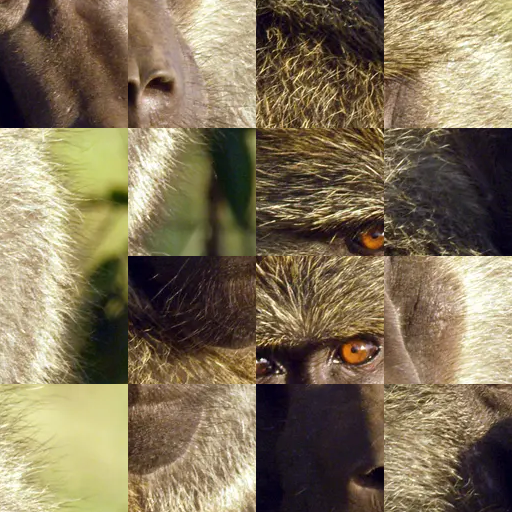
\includegraphics[width=6cm]{resultados/colormsc.png}
        \caption{\texttt{imagens/color.png}}
    \end{subfigure}%
    \begin{subfigure}{0.45\textwidth}
        \centering
        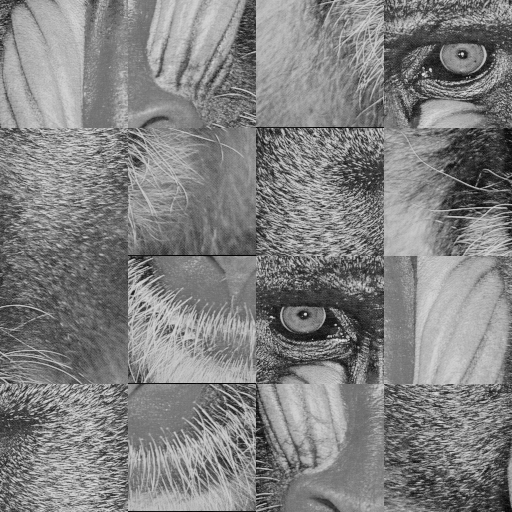
\includegraphics[width=6cm]{resultados/baboonmsc.png}
        \caption{\texttt{imagens/babooon.png}}
        \label{fig:res:10}
    \end{subfigure}

    \caption{Mosaico da imagem com \textcolor{red}{ALGUMA COISA}.}
\end{figure}

\begin{listing}[H]
    \begin{minted}{python}
        def mosaico(imagem, ordem):
            N, M = ordem.shape
            # split e flatten
            bloco = [
                bloco
                for lin in np.vsplit(imagem, N)
                for bloco in np.hsplit(lin, M)
            ]
            # accesso (em lista) e concatena
            imagem = np.concatenate([
                np.concatenate([bloco[i] for i in lin], axis=1)
                for lin in ordem
            ])
            return imagem
    \end{minted}

    \caption{Comando \texttt{mosaico ORDENACAO}}
\end{listing}
